\documentclass[14pt]{extbook}
\usepackage{multicol, enumerate, enumitem, hyperref, color, soul, setspace, parskip, fancyhdr} %General Packages
\usepackage{amssymb, amsthm, amsmath, bbm, latexsym, units, mathtools} %Math Packages
\everymath{\displaystyle} %All math in Display Style
% Packages with additional options
\usepackage[headsep=0.5cm,headheight=12pt, left=1 in,right= 1 in,top= 1 in,bottom= 1 in]{geometry}
\usepackage[usenames,dvipsnames]{xcolor}
\usepackage{dashrule}  % Package to use the command below to create lines between items
\newcommand{\litem}[1]{\item#1\hspace*{-1cm}\rule{\textwidth}{0.4pt}}
\pagestyle{fancy}
\lhead{Progress Quiz 10}
\chead{}
\rhead{Version C}
\lfoot{6232-9639}
\cfoot{}
\rfoot{Fall 2020}
\begin{document}

\begin{enumerate}
\litem{
First, find the equation of the line containing the two points below. Then, write the equation as $ y=mx+b $ and choose the intervals that contain $m$ and $b$.\[ (9, 11) \text{ and } (2, 7) \]\begin{enumerate}[label=\Alph*.]
\item \( m \in [0.4, 3.9] \hspace*{3mm} b \in [-6.93, -5.19] \)
\item \( m \in [0.4, 3.9] \hspace*{3mm} b \in [4.54, 5.31] \)
\item \( m \in [0.4, 3.9] \hspace*{3mm} b \in [0.45, 3.86] \)
\item \( m \in [-2.6, -0.2] \hspace*{3mm} b \in [7.47, 10.38] \)
\item \( m \in [0.4, 3.9] \hspace*{3mm} b \in [5.09, 6.45] \)

\end{enumerate} }
\litem{
Find the equation of the line described below. Write the linear equation as $ y=mx+b $ and choose the intervals that contain $m$ and $b$.\[ \text{Parallel to } 5 x + 3 y = 9 \text{ and passing through the point } (-5, -6). \]\begin{enumerate}[label=\Alph*.]
\item \( m \in [-3.7, -1.3] \hspace*{3mm} b \in [-18.33, -13.33] \)
\item \( m \in [0.6, 2.5] \hspace*{3mm} b \in [1.33, 8.33] \)
\item \( m \in [-1.6, 0.8] \hspace*{3mm} b \in [-18.33, -13.33] \)
\item \( m \in [-3.7, -1.3] \hspace*{3mm} b \in [-3, 0] \)
\item \( m \in [-3.7, -1.3] \hspace*{3mm} b \in [11.33, 16.33] \)

\end{enumerate} }
\litem{
Find the equation of the line described below. Write the linear equation as $ y=mx+b $ and choose the intervals that contain $m$ and $b$.\[ \text{Perpendicular to } 7 x + 9 y = 8 \text{ and passing through the point } (-3, -5). \]\begin{enumerate}[label=\Alph*.]
\item \( m \in [1.12, 1.68] \hspace*{3mm} b \in [-2.5, -1.45] \)
\item \( m \in [0.75, 1.05] \hspace*{3mm} b \in [-1.93, -0.4] \)
\item \( m \in [-1.6, -0.69] \hspace*{3mm} b \in [-9.91, -8.29] \)
\item \( m \in [1.12, 1.68] \hspace*{3mm} b \in [0.62, 2.3] \)
\item \( m \in [1.12, 1.68] \hspace*{3mm} b \in [-1.93, -0.4] \)

\end{enumerate} }
\litem{
First, find the equation of the line containing the two points below. Then, write the equation as $ y=mx+b $ and choose the intervals that contain $m$ and $b$.\[ (-5, -11) \text{ and } (9, 6) \]\begin{enumerate}[label=\Alph*.]
\item \( m \in [0.21, 7.21] \hspace*{3mm} b \in [-4.17, -2.94] \)
\item \( m \in [0.21, 7.21] \hspace*{3mm} b \in [-5.13, -4.16] \)
\item \( m \in [0.21, 7.21] \hspace*{3mm} b \in [3.37, 5.08] \)
\item \( m \in [0.21, 7.21] \hspace*{3mm} b \in [-7.23, -5.22] \)
\item \( m \in [-3.21, -0.21] \hspace*{3mm} b \in [16.45, 17.98] \)

\end{enumerate} }
\litem{
Write the equation of the line in the graph below in Standard form $Ax+By=C$. Then, choose the intervals that contain $A, B, \text{ and } C$.
\begin{center}
    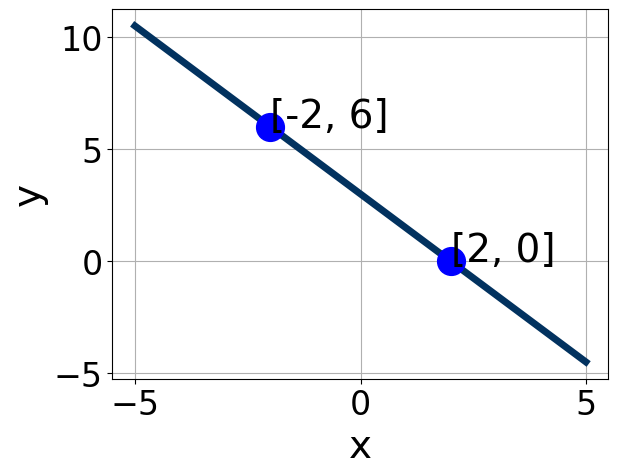
\includegraphics[width=0.5\textwidth]{../Figures/linearGraphToStandardCopyC.png}
\end{center}
\begin{enumerate}[label=\Alph*.]
\item \( A \in [1.9, 4.5], \hspace{3mm} B \in [1.56, 2.01], \text{ and } \hspace{3mm} C \in [5.2, 7.3] \)
\item \( A \in [1.1, 2.3], \hspace{3mm} B \in [-1.32, -0.27], \text{ and } \hspace{3mm} C \in [-3.2, -1.7] \)
\item \( A \in [1.9, 4.5], \hspace{3mm} B \in [-2.06, -1.79], \text{ and } \hspace{3mm} C \in [-6.8, -4.4] \)
\item \( A \in [1.1, 2.3], \hspace{3mm} B \in [0.77, 1.29], \text{ and } \hspace{3mm} C \in [0.2, 4.5] \)
\item \( A \in [-3.5, -2.2], \hspace{3mm} B \in [-2.06, -1.79], \text{ and } \hspace{3mm} C \in [-6.8, -4.4] \)

\end{enumerate} }
\litem{
Solve the equation below. Then, choose the interval that contains the solution.\[ -19(-14x + 6) = -18(10x + 7) \]\begin{enumerate}[label=\Alph*.]
\item \( x \in [-0.63, -0.32] \)
\item \( x \in [2.4, 2.82] \)
\item \( x \in [-0.26, 0.19] \)
\item \( x \in [0.03, 0.77] \)
\item \( \text{There are no real solutions.} \)

\end{enumerate} }
\litem{
Solve the linear equation below. Then, choose the interval that contains the solution.\[ \frac{-3x + 6}{5} - \frac{-3x + 9}{4} = \frac{4x + 7}{7} \]\begin{enumerate}[label=\Alph*.]
\item \( x \in [-8.86, -1.86] \)
\item \( x \in [-2.51, 3.49] \)
\item \( x \in [-24.73, -20.73] \)
\item \( x \in [5.81, 7.81] \)
\item \( \text{There are no real solutions.} \)

\end{enumerate} }
\litem{
Solve the linear equation below. Then, choose the interval that contains the solution.\[ \frac{9x -7}{5} - \frac{-7x -4}{8} = \frac{7x + 7}{3} \]\begin{enumerate}[label=\Alph*.]
\item \( x \in [25.27, 30.27] \)
\item \( x \in [-1.64, 4.36] \)
\item \( x \in [12.39, 13.39] \)
\item \( x \in [9.46, 11.46] \)
\item \( \text{There are no real solutions.} \)

\end{enumerate} }
\litem{
Write the equation of the line in the graph below in Standard form $Ax+By=C$. Then, choose the intervals that contain $A, B, \text{ and } C$.
\begin{center}
    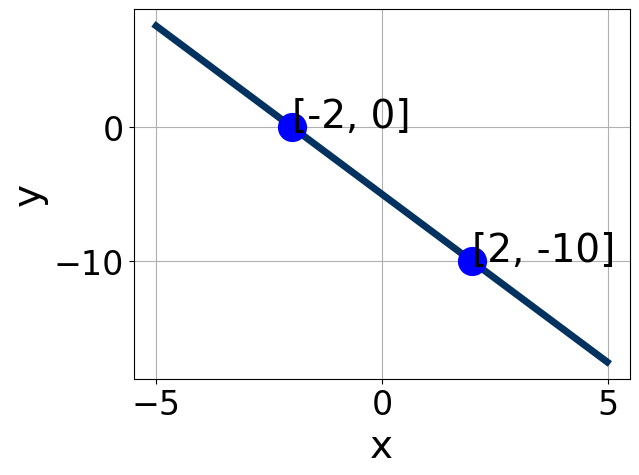
\includegraphics[width=0.5\textwidth]{../Figures/linearGraphToStandardC.png}
\end{center}
\begin{enumerate}[label=\Alph*.]
\item \( A \in [3, 11], \hspace{3mm} B \in [1.78, 3.49], \text{ and } \hspace{3mm} C \in [-10.6, -8.3] \)
\item \( A \in [-6, 2], \hspace{3mm} B \in [-2.02, -1.55], \text{ and } \hspace{3mm} C \in [9.8, 11.3] \)
\item \( A \in [3, 11], \hspace{3mm} B \in [-2.02, -1.55], \text{ and } \hspace{3mm} C \in [9.8, 11.3] \)
\item \( A \in [2.5, 3.5], \hspace{3mm} B \in [0.86, 1.02], \text{ and } \hspace{3mm} C \in [-6.5, -4.5] \)
\item \( A \in [2.5, 3.5], \hspace{3mm} B \in [-1.42, 0.16], \text{ and } \hspace{3mm} C \in [3.7, 5.6] \)

\end{enumerate} }
\litem{
Solve the equation below. Then, choose the interval that contains the solution.\[ -13(-19x + 11) = -5(-7x -12) \]\begin{enumerate}[label=\Alph*.]
\item \( x \in [0.95, 1.06] \)
\item \( x \in [0.23, 0.39] \)
\item \( x \in [-0.45, -0.28] \)
\item \( x \in [0.3, 0.6] \)
\item \( \text{There are no real solutions.} \)

\end{enumerate} }
\end{enumerate}

\end{document}